\chapter{Исследовательская часть}

\section{Технические характеристики}
Характеристики используемого оборудования:
\begin{itemize}
    \item Операционная система --- Windows 11 Home [3]
    \item Память --- 16 Гб.
    \item Процессор --- Intel(R) Core(TM) i5-10300H CPU @ 2.50Ггц [4]
\end{itemize}

\section{Описание используемых типов данных}
Используемые типы данных:
\begin{itemize}
	\item словарь --- массив из $N$ различных элементов типа $int$;
	\item искомый элемент --- число типа $int$.
\end{itemize}

\section{Гистограммы}

На рисунках \ref{fig:diag-1} --- \ref{fig:diag-3} приведены гистограммы, показывающие количество сравнений для каждого элемента словаря в трех вариациях:
\begin{itemize}
    \item используется алгоритм полного перебора;
    \item используется алгоритм бинарного поиска на упорядоченном массиве;
    \item вторая вариация, где столбцы упорядочены в порядке возрастания.
\end{itemize}

\begin{figure}
    \centering
    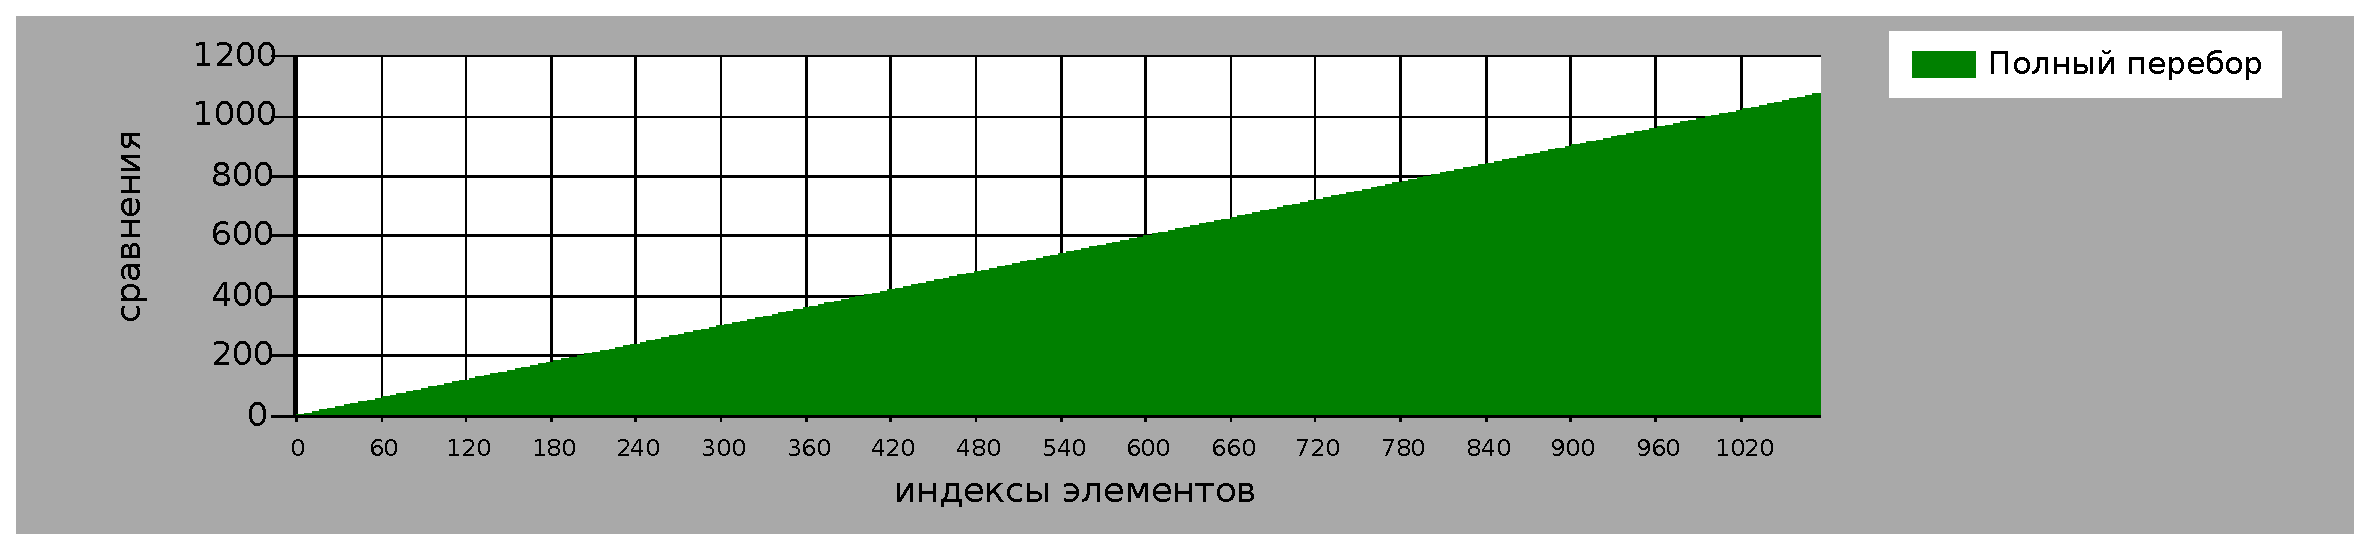
\includegraphics[width=1\linewidth]{img/chart1.eps}
    \caption{Сравнения для каждого элемента в алгоритме полного перебора}
    \label{fig:diag-1}
\end{figure}

\begin{figure}
    \centering
    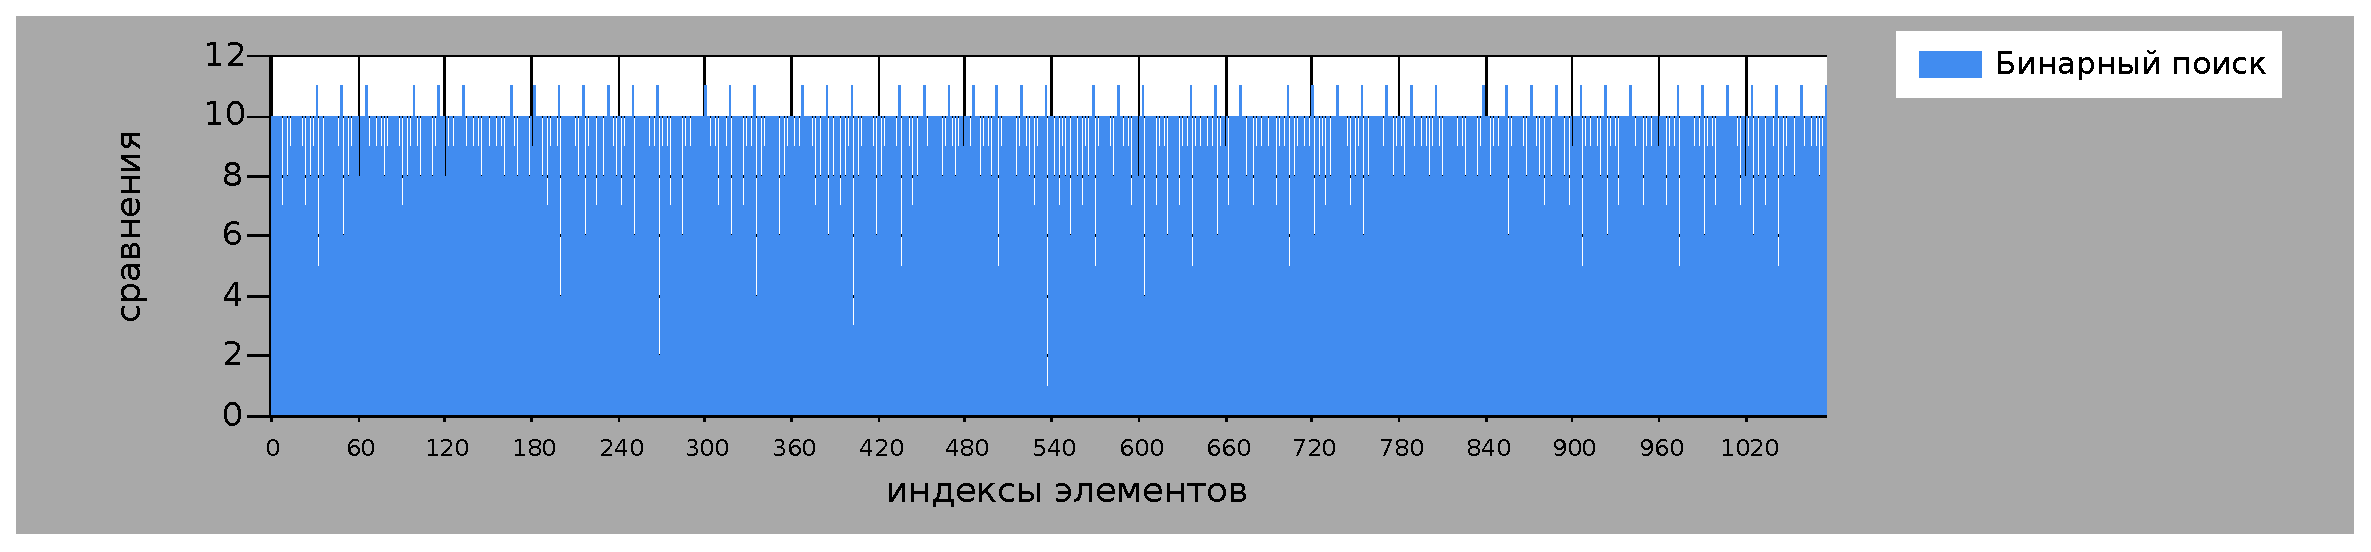
\includegraphics[width=1\linewidth]{img/chart2.eps}
    \caption{Сравнения для каждого элемента в алгоритме бинарного поиска}
    \label{fig:diag-2}
\end{figure}

\begin{figure}
    \centering
    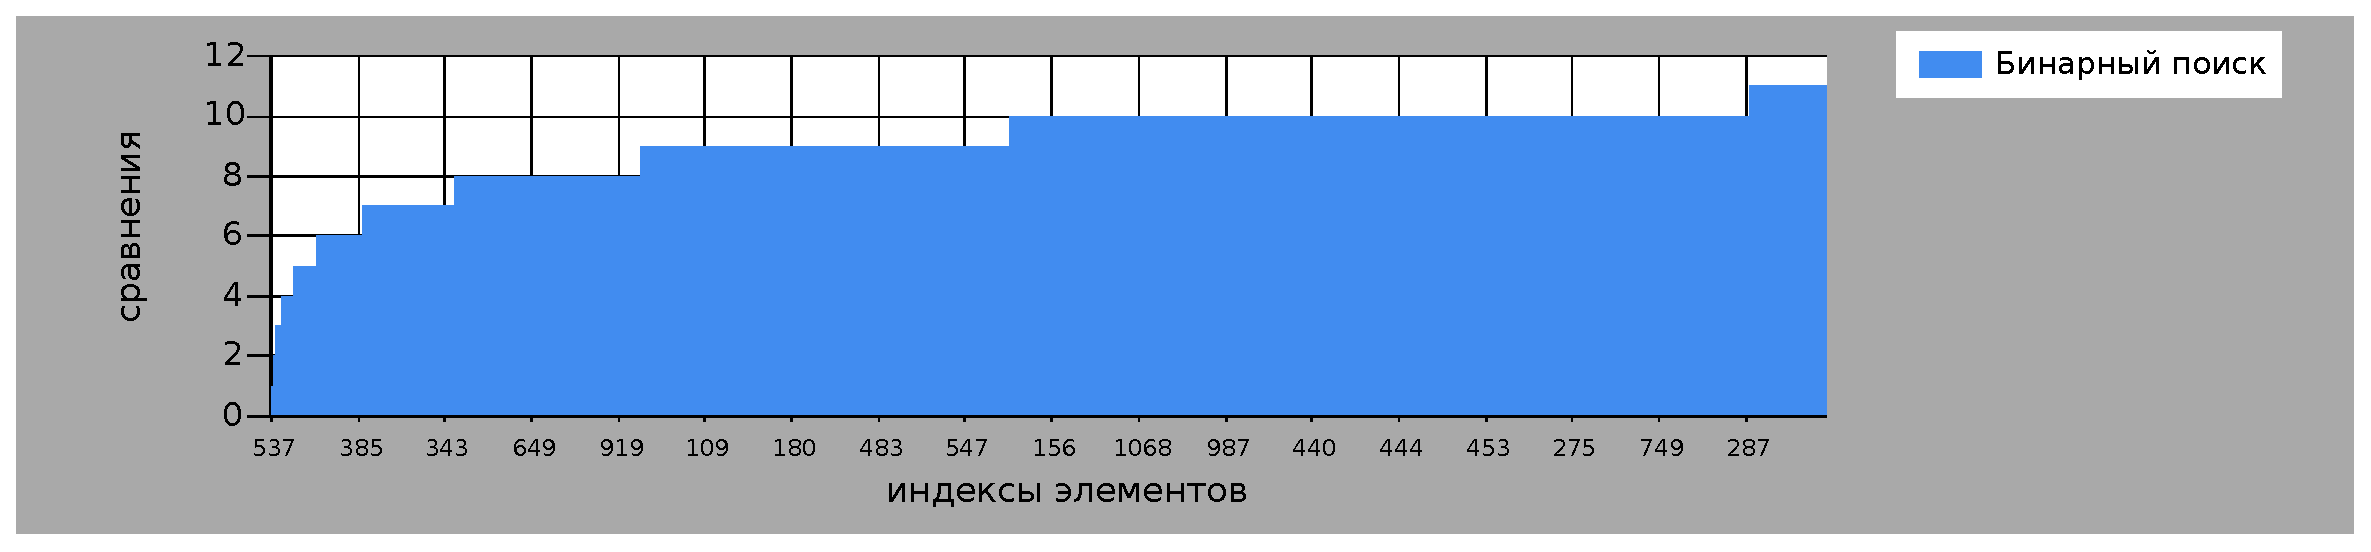
\includegraphics[width=1\linewidth]{img/chart3.eps}
    \caption{Сравнения для каждого элемента в алгоритме полного перебора (отсортирован)}
    \label{fig:diag-3}
\end{figure}

\clearpage

% \section{Оценка памяти}

% Рекурсивная версия алгоритма Левенштейна не использует явных структур данных для хранения промежуточных вычислений. Вместо этого каждый вызов функции обрабатывает небольшой фрагмент строк, и функция вызывает саму себя несколько раз. Глубина рекурсии в худшем случае составляет: 
% \begin{equation}
% 	(len(S_{1}) + len(S_{2})).
% \end{equation}
% При этом каждый рекурсивный вызов требует хранения локальных переменных: 2 переменные типа $int$, 2 переменные типа $str$. В результате, максимальный расход памяти составляет:
% \begin{equation}
% 	(len(S_{1}) + len(S_{2})) \cdot (2 \cdot size(\text{int}) + 2 \cdot size(\text{str})),
% \end{equation}
% где $size$ - функция, вычисляющая размер параметра.

% Алгоритм, основанный на динамическом программировании, использует двумерную матрицу размером $len(S_{1} + 1) \times len(S_{2} + 1)$
% Эта матрица хранит результаты всех промежуточных вычислений (расстояние Левенштейна для всех подстрок). Дополнительно хранятся локальные переменные: 5 переменных типа $int$, 2 переменные типа $str$. По итогу расход памяти в данном случае составляет:
% \begin{equation}
% 	(len(S_{1} + 1) \cdot len(S_{2} + 1) \cdot size(\text{int})) + 5 \cdot size(\text{int}) + 2 \cdot size(\text{str})).
% \end{equation}

% По расходу памяти алгоритм, использующий принцип динамического программирования, проигрывает рекурсивному: максимальный размер используемой памяти в них растёт как произведение длин строк, в то время как у рекурсивного алгоритма — как сумма длин строк.

% Алгоритм Дамерау-Левенштейна, также реализованный через динамическое программирование, аналогичен по своей структуре алгоритму Левенштейна. Основное отличие заключается в дополнительной проверке для учёта операций перестановки соседних символов. Для этого используется та же матрица размера 
% $len(S_{1} + 1) \times (len(S_{2} + 1)$
% , что и в динамическом алгоритме Левенштейна.

% Несмотря на добавление новой операции (перестановка), использование памяти остаётся также на уровне 
% произведение длин строк, поскольку не требуется дополнительное пространство для хранения результатов перестановок. Как и в случае с Левенштейном, каждая клетка матрицы заполняется лишь однажды.

% \clearpage

% \section{Время выполнения алгоритмов}
% Результаты замеров времени работы трех алгоритмов умножения матриц приведены в таблице \ref{tbl:time_measurements}. Замеры времени проводились на матрицах одинаковой длины и усреднялись для каждого набора одинаковых экспериментов. Каждое значение получено путем взятия среднего из 100 измерений.

% \begin{table}[h]
% 	\begin{center}
% 		\begin{threeparttable}
% 		\captionsetup{justification=raggedright,singlelinecheck=off}
% 		\caption{Время работы алгоритмов (в мс)}
% 		\label{tbl:time_measurements}
% 		\begin{tabular}{|c|c|c|c|c|}
% 			\hline
% 			Размер матрицы &  Классич. & Вин. & Вин. опт. \\
%             \hline
% 			1    & 0.01 & 0.00 & 0.00 \\
%             \hline
% 			2    & 0.01 & 0.02 & 0.00 \\ 
%             \hline
% 			4    & 0.02 & 0.04 & 0.04 \\ 
%             \hline
% 			8    & 0.04 & 0.05 & 0.06 \\ 
% 			\hline
% 			10    & 0.09 & 0.05 & 0.04 \\ 
% 			\hline
% 			20    & 0.37 & 0.31 & 0.43 \\ 
% 			\hline
% 			30    & 1.23 & 1.18 & 0.87 \\ 
% 			\hline
% 			40    & 3.20 & 2.77 & 2.22 \\ 
% 			\hline
% 			50    & 5.96 & 5.14 & 3.96 \\ 
% 			\hline
% 			60    & 10.25 & 8.87 & 6.98 \\ 
% 			\hline
% 			70    & 16.20 & 14.05 & 10.92 \\ 
% 			\hline
%             80    & 24.12 & 20.71 & 16.37 \\ 
%             \hline
%             90    & 34.18 & 29.00 & 22.84 \\ 
%             \hline
%             100    & 46.90 & 40.19 & 31.68 \\ 
%             \hline
% 		\end{tabular}
% 		\end{threeparttable}
%     \end{center}
% \end{table}

% \begin{figure}[H]
%     \centering
%     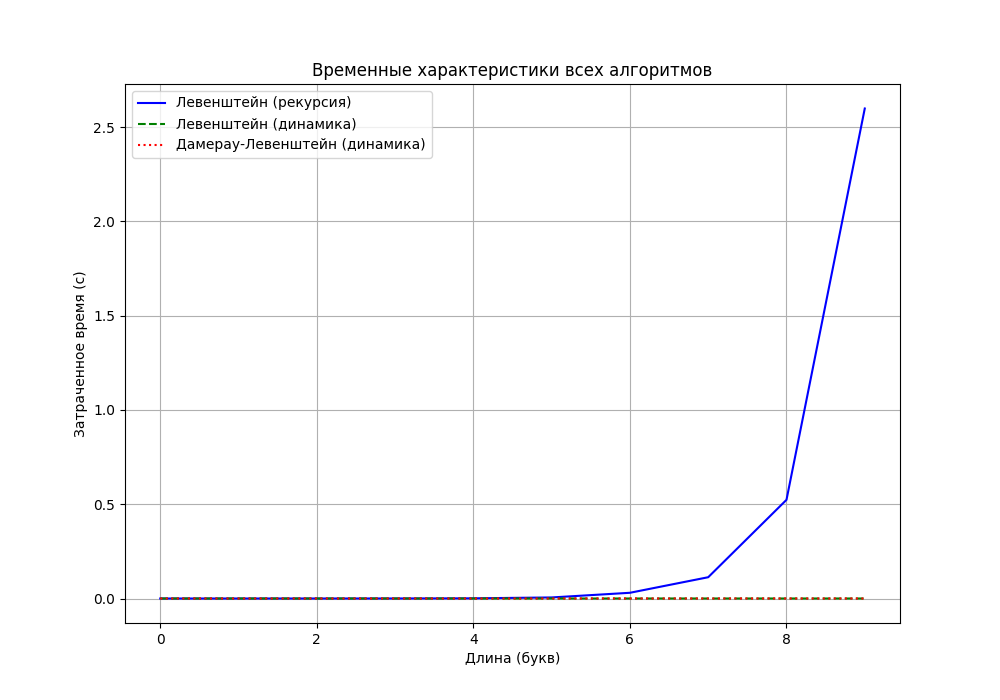
\includegraphics[width=0.8\linewidth]{img/Figure_3.png}
%     \vspace{5mm}
%     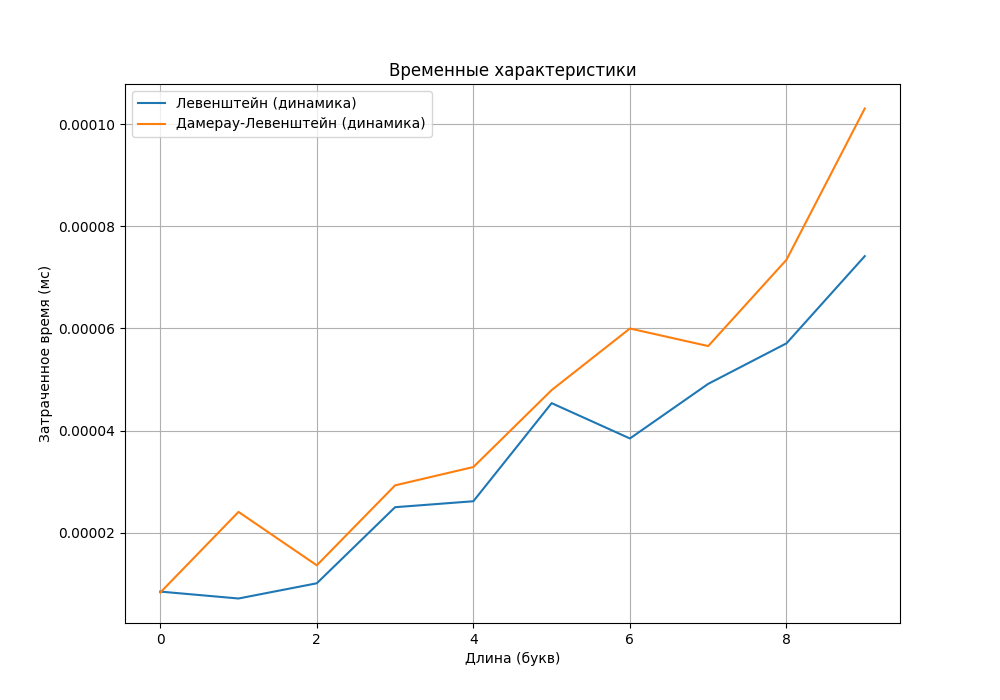
\includegraphics[width=0.8\linewidth]{img/Figure_2.png}
%     \caption{Сравнение алгоритмов по времени}
%     \label{fig:time_measurements}
% \end{figure}

% \clearpage

\section{Вывод}
На основе полученных гистограмм для двух алгоритмов поиска в массиве (полного перебора и бинарного поиска) можно сделать следующие выводы:

\textbf{Полный перебор:}
\begin{itemize}
    \item В лучшем случае, если искомый элемент находится в начале массива, алгоритм выполняет минимальное количество операций, что соответствует трудоемкости $O(1)$.
    \item Гистограмма показала, что трудоемкость алгоритма линейно растет с увеличением индекса элемента, который необходимо найти. Это подтверждает теоретическую оценку трудоемкости $O(N)$ в худшем случае.
\end{itemize}

\textbf{Бинарный поиск:}
\begin{itemize}
    \item В лучшем случае, если элемент находится в середине массива, бинарный поиск завершает работу, что соответствует трудоемкости $O(1)$.
    \item Гистограмма для бинарного поиска демонстрирует гораздо меньшую трудоемкость по сравнению с полным перебором (почти в $100$ раз меньше сравнений для худшего случая). Количество операций увеличивается логарифмически, что соответствует трудоемкости $O(\log N)$.
\end{itemize}